\documentclass{ximera}

%\usepackage{todonotes}
%\usepackage{mathtools} %% Required for wide table Curl and Greens
%\usepackage{cuted} %% Required for wide table Curl and Greens
\newcommand{\todo}{}

\usepackage{esint} % for \oiint
\ifxake%%https://math.meta.stackexchange.com/questions/9973/how-do-you-render-a-closed-surface-double-integral
\renewcommand{\oiint}{{\large\bigcirc}\kern-1.56em\iint}
\fi


\graphicspath{
  {./}
  {ximeraTutorial/}
  {basicPhilosophy/}
  {functionsOfSeveralVariables/}
  {normalVectors/}
  {lagrangeMultipliers/}
  {vectorFields/}
  {greensTheorem/}
  {shapeOfThingsToCome/}
  {dotProducts/}
  {partialDerivativesAndTheGradientVector/}
  {../productAndQuotientRules/exercises/}
  {../normalVectors/exercisesParametricPlots/}
  {../continuityOfFunctionsOfSeveralVariables/exercises/}
  {../partialDerivativesAndTheGradientVector/exercises/}
  {../directionalDerivativeAndChainRule/exercises/}
  {../commonCoordinates/exercisesCylindricalCoordinates/}
  {../commonCoordinates/exercisesSphericalCoordinates/}
  {../greensTheorem/exercisesCurlAndLineIntegrals/}
  {../greensTheorem/exercisesDivergenceAndLineIntegrals/}
  {../shapeOfThingsToCome/exercisesDivergenceTheorem/}
  {../greensTheorem/}
  {../shapeOfThingsToCome/}
  {../separableDifferentialEquations/exercises/}
  {vectorFields/}
}

\newcommand{\mooculus}{\textsf{\textbf{MOOC}\textnormal{\textsf{ULUS}}}}

\usepackage{tkz-euclide}\usepackage{tikz}
\usepackage{tikz-cd}
\usetikzlibrary{arrows}
\tikzset{>=stealth,commutative diagrams/.cd,
  arrow style=tikz,diagrams={>=stealth}} %% cool arrow head
\tikzset{shorten <>/.style={ shorten >=#1, shorten <=#1 } } %% allows shorter vectors

\usetikzlibrary{backgrounds} %% for boxes around graphs
\usetikzlibrary{shapes,positioning}  %% Clouds and stars
\usetikzlibrary{matrix} %% for matrix
\usepgfplotslibrary{polar} %% for polar plots
\usepgfplotslibrary{fillbetween} %% to shade area between curves in TikZ
\usetkzobj{all}
\usepackage[makeroom]{cancel} %% for strike outs
%\usepackage{mathtools} %% for pretty underbrace % Breaks Ximera
%\usepackage{multicol}
\usepackage{pgffor} %% required for integral for loops



%% http://tex.stackexchange.com/questions/66490/drawing-a-tikz-arc-specifying-the-center
%% Draws beach ball
\tikzset{pics/carc/.style args={#1:#2:#3}{code={\draw[pic actions] (#1:#3) arc(#1:#2:#3);}}}



\usepackage{array}
\setlength{\extrarowheight}{+.1cm}
\newdimen\digitwidth
\settowidth\digitwidth{9}
\def\divrule#1#2{
\noalign{\moveright#1\digitwidth
\vbox{\hrule width#2\digitwidth}}}





\newcommand{\RR}{\mathbb R}
\newcommand{\R}{\mathbb R}
\newcommand{\N}{\mathbb N}
\newcommand{\Z}{\mathbb Z}

\newcommand{\sagemath}{\textsf{SageMath}}


%\renewcommand{\d}{\,d\!}
\renewcommand{\d}{\mathop{}\!d}
\newcommand{\dd}[2][]{\frac{\d #1}{\d #2}}
\newcommand{\pp}[2][]{\frac{\partial #1}{\partial #2}}
\renewcommand{\l}{\ell}
\newcommand{\ddx}{\frac{d}{\d x}}

\newcommand{\zeroOverZero}{\ensuremath{\boldsymbol{\tfrac{0}{0}}}}
\newcommand{\inftyOverInfty}{\ensuremath{\boldsymbol{\tfrac{\infty}{\infty}}}}
\newcommand{\zeroOverInfty}{\ensuremath{\boldsymbol{\tfrac{0}{\infty}}}}
\newcommand{\zeroTimesInfty}{\ensuremath{\small\boldsymbol{0\cdot \infty}}}
\newcommand{\inftyMinusInfty}{\ensuremath{\small\boldsymbol{\infty - \infty}}}
\newcommand{\oneToInfty}{\ensuremath{\boldsymbol{1^\infty}}}
\newcommand{\zeroToZero}{\ensuremath{\boldsymbol{0^0}}}
\newcommand{\inftyToZero}{\ensuremath{\boldsymbol{\infty^0}}}



\newcommand{\numOverZero}{\ensuremath{\boldsymbol{\tfrac{\#}{0}}}}
\newcommand{\dfn}{\textbf}
%\newcommand{\unit}{\,\mathrm}
\newcommand{\unit}{\mathop{}\!\mathrm}
\newcommand{\eval}[1]{\bigg[ #1 \bigg]}
\newcommand{\seq}[1]{\left( #1 \right)}
\renewcommand{\epsilon}{\varepsilon}
\renewcommand{\phi}{\varphi}


\renewcommand{\iff}{\Leftrightarrow}

\DeclareMathOperator{\arccot}{arccot}
\DeclareMathOperator{\arcsec}{arcsec}
\DeclareMathOperator{\arccsc}{arccsc}
\DeclareMathOperator{\si}{Si}
\DeclareMathOperator{\scal}{scal}
\DeclareMathOperator{\sign}{sign}


%% \newcommand{\tightoverset}[2]{% for arrow vec
%%   \mathop{#2}\limits^{\vbox to -.5ex{\kern-0.75ex\hbox{$#1$}\vss}}}
\newcommand{\arrowvec}[1]{{\overset{\rightharpoonup}{#1}}}
%\renewcommand{\vec}[1]{\arrowvec{\mathbf{#1}}}
\renewcommand{\vec}[1]{{\overset{\boldsymbol{\rightharpoonup}}{\mathbf{#1}}}\hspace{0in}}

\newcommand{\point}[1]{\left(#1\right)} %this allows \vector{ to be changed to \vector{ with a quick find and replace
\newcommand{\pt}[1]{\mathbf{#1}} %this allows \vec{ to be changed to \vec{ with a quick find and replace
\newcommand{\Lim}[2]{\lim_{\point{#1} \to \point{#2}}} %Bart, I changed this to point since I want to use it.  It runs through both of the exercise and exerciseE files in limits section, which is why it was in each document to start with.

\DeclareMathOperator{\proj}{\mathbf{proj}}
\newcommand{\veci}{{\boldsymbol{\hat{\imath}}}}
\newcommand{\vecj}{{\boldsymbol{\hat{\jmath}}}}
\newcommand{\veck}{{\boldsymbol{\hat{k}}}}
\newcommand{\vecl}{\vec{\boldsymbol{\l}}}
\newcommand{\uvec}[1]{\mathbf{\hat{#1}}}
\newcommand{\utan}{\mathbf{\hat{t}}}
\newcommand{\unormal}{\mathbf{\hat{n}}}
\newcommand{\ubinormal}{\mathbf{\hat{b}}}

\newcommand{\dotp}{\bullet}
\newcommand{\cross}{\boldsymbol\times}
\newcommand{\grad}{\boldsymbol\nabla}
\newcommand{\divergence}{\grad\dotp}
\newcommand{\curl}{\grad\cross}
%\DeclareMathOperator{\divergence}{divergence}
%\DeclareMathOperator{\curl}[1]{\grad\cross #1}
\newcommand{\lto}{\mathop{\longrightarrow\,}\limits}

\renewcommand{\bar}{\overline}

\colorlet{textColor}{black}
\colorlet{background}{white}
\colorlet{penColor}{blue!50!black} % Color of a curve in a plot
\colorlet{penColor2}{red!50!black}% Color of a curve in a plot
\colorlet{penColor3}{red!50!blue} % Color of a curve in a plot
\colorlet{penColor4}{green!50!black} % Color of a curve in a plot
\colorlet{penColor5}{orange!80!black} % Color of a curve in a plot
\colorlet{penColor6}{yellow!70!black} % Color of a curve in a plot
\colorlet{fill1}{penColor!20} % Color of fill in a plot
\colorlet{fill2}{penColor2!20} % Color of fill in a plot
\colorlet{fillp}{fill1} % Color of positive area
\colorlet{filln}{penColor2!20} % Color of negative area
\colorlet{fill3}{penColor3!20} % Fill
\colorlet{fill4}{penColor4!20} % Fill
\colorlet{fill5}{penColor5!20} % Fill
\colorlet{gridColor}{gray!50} % Color of grid in a plot

\newcommand{\surfaceColor}{violet}
\newcommand{\surfaceColorTwo}{redyellow}
\newcommand{\sliceColor}{greenyellow}




\pgfmathdeclarefunction{gauss}{2}{% gives gaussian
  \pgfmathparse{1/(#2*sqrt(2*pi))*exp(-((x-#1)^2)/(2*#2^2))}%
}


%%%%%%%%%%%%%
%% Vectors
%%%%%%%%%%%%%

%% Simple horiz vectors
\renewcommand{\vector}[1]{\left\langle #1\right\rangle}


%% %% Complex Horiz Vectors with angle brackets
%% \makeatletter
%% \renewcommand{\vector}[2][ , ]{\left\langle%
%%   \def\nextitem{\def\nextitem{#1}}%
%%   \@for \el:=#2\do{\nextitem\el}\right\rangle%
%% }
%% \makeatother

%% %% Vertical Vectors
%% \def\vector#1{\begin{bmatrix}\vecListA#1,,\end{bmatrix}}
%% \def\vecListA#1,{\if,#1,\else #1\cr \expandafter \vecListA \fi}

%%%%%%%%%%%%%
%% End of vectors
%%%%%%%%%%%%%

%\newcommand{\fullwidth}{}
%\newcommand{\normalwidth}{}



%% makes a snazzy t-chart for evaluating functions
%\newenvironment{tchart}{\rowcolors{2}{}{background!90!textColor}\array}{\endarray}

%%This is to help with formatting on future title pages.
\newenvironment{sectionOutcomes}{}{}



%% Flowchart stuff
%\tikzstyle{startstop} = [rectangle, rounded corners, minimum width=3cm, minimum height=1cm,text centered, draw=black]
%\tikzstyle{question} = [rectangle, minimum width=3cm, minimum height=1cm, text centered, draw=black]
%\tikzstyle{decision} = [trapezium, trapezium left angle=70, trapezium right angle=110, minimum width=3cm, minimum height=1cm, text centered, draw=black]
%\tikzstyle{question} = [rectangle, rounded corners, minimum width=3cm, minimum height=1cm,text centered, draw=black]
%\tikzstyle{process} = [rectangle, minimum width=3cm, minimum height=1cm, text centered, draw=black]
%\tikzstyle{decision} = [trapezium, trapezium left angle=70, trapezium right angle=110, minimum width=3cm, minimum height=1cm, text centered, draw=black]


\title[Dig-In:]{Parametric plots}

\begin{document}
\begin{abstract}
  Tangent and normal vectors can help us plot make interesting
  parametric functions.
\end{abstract}
\maketitle

\section{A sine curve on a circle}

Suppose you wish to make a sine curve on a circle like this:
\begin{image}
  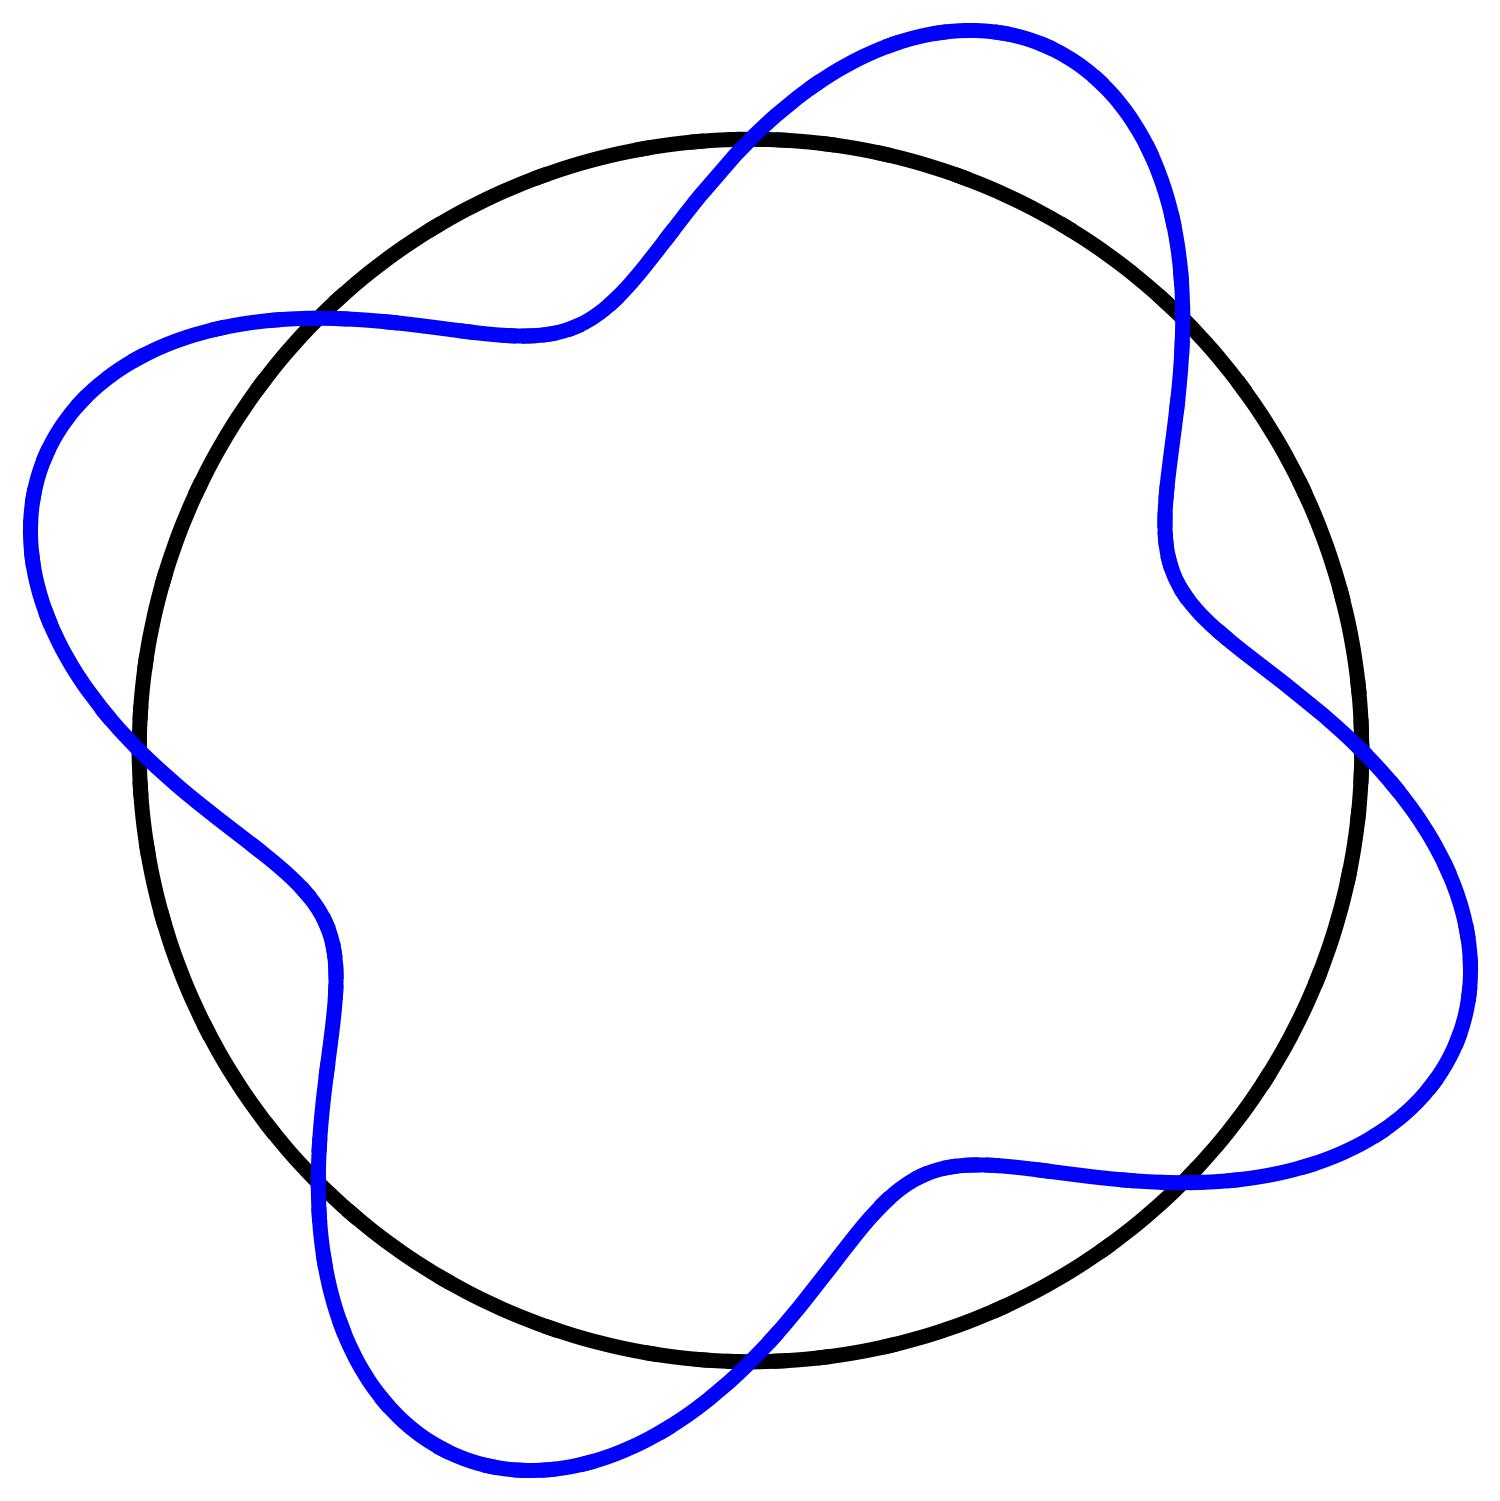
\includegraphics{sinOnCircle.jpg}
\end{image}

How do you do this? You will use unit tangent and unit normal vectors!
\begin{example}
  Plot the curve $y= \sin(5x)$ ``wrapped'' around a circle of radius $3$.
  \begin{explanation}
    To do this, start by setting
    \[
    \vec{c}(t) = \vector{3\cos(t),\answer[given]{3\sin(t)}}
    \]
    This will produce our circle of radius $3$.
\begin{onlineOnly}
\begin{sageCell}
var('s t')
x(t) = 3*cos(t)
y(t) = 3*sin(t)
c(t) = (x(t),y(t))
circle=parametric_plot(c(t),(t,0,2*pi),color="black")
circle
\end{sageCell}
\end{onlineOnly}
Now we need to add our sine curve. To do this, we compute the unit tangent vector
\begin{align*}
  \utan(t) &= \frac{\vec{c}'(t)}{|\vec{c}'(t)|}\\
  &=\vector{\answer[given]{-\sin(t)},\answer[given]{\cos(t)}}
\end{align*}
and the unit normal vector:
\begin{align*}
  \unormal(t) &= \frac{\utan'(t)}{|\utan'(t)|}\\
  &=\vector{\answer[given]{-\cos(t)},\answer[given]{-\sin(t)}}
\end{align*}
We've plotted our circle of radius $3$ with some unit tangent and unit
normal vectors for your viewing pleasure:
\begin{image}
  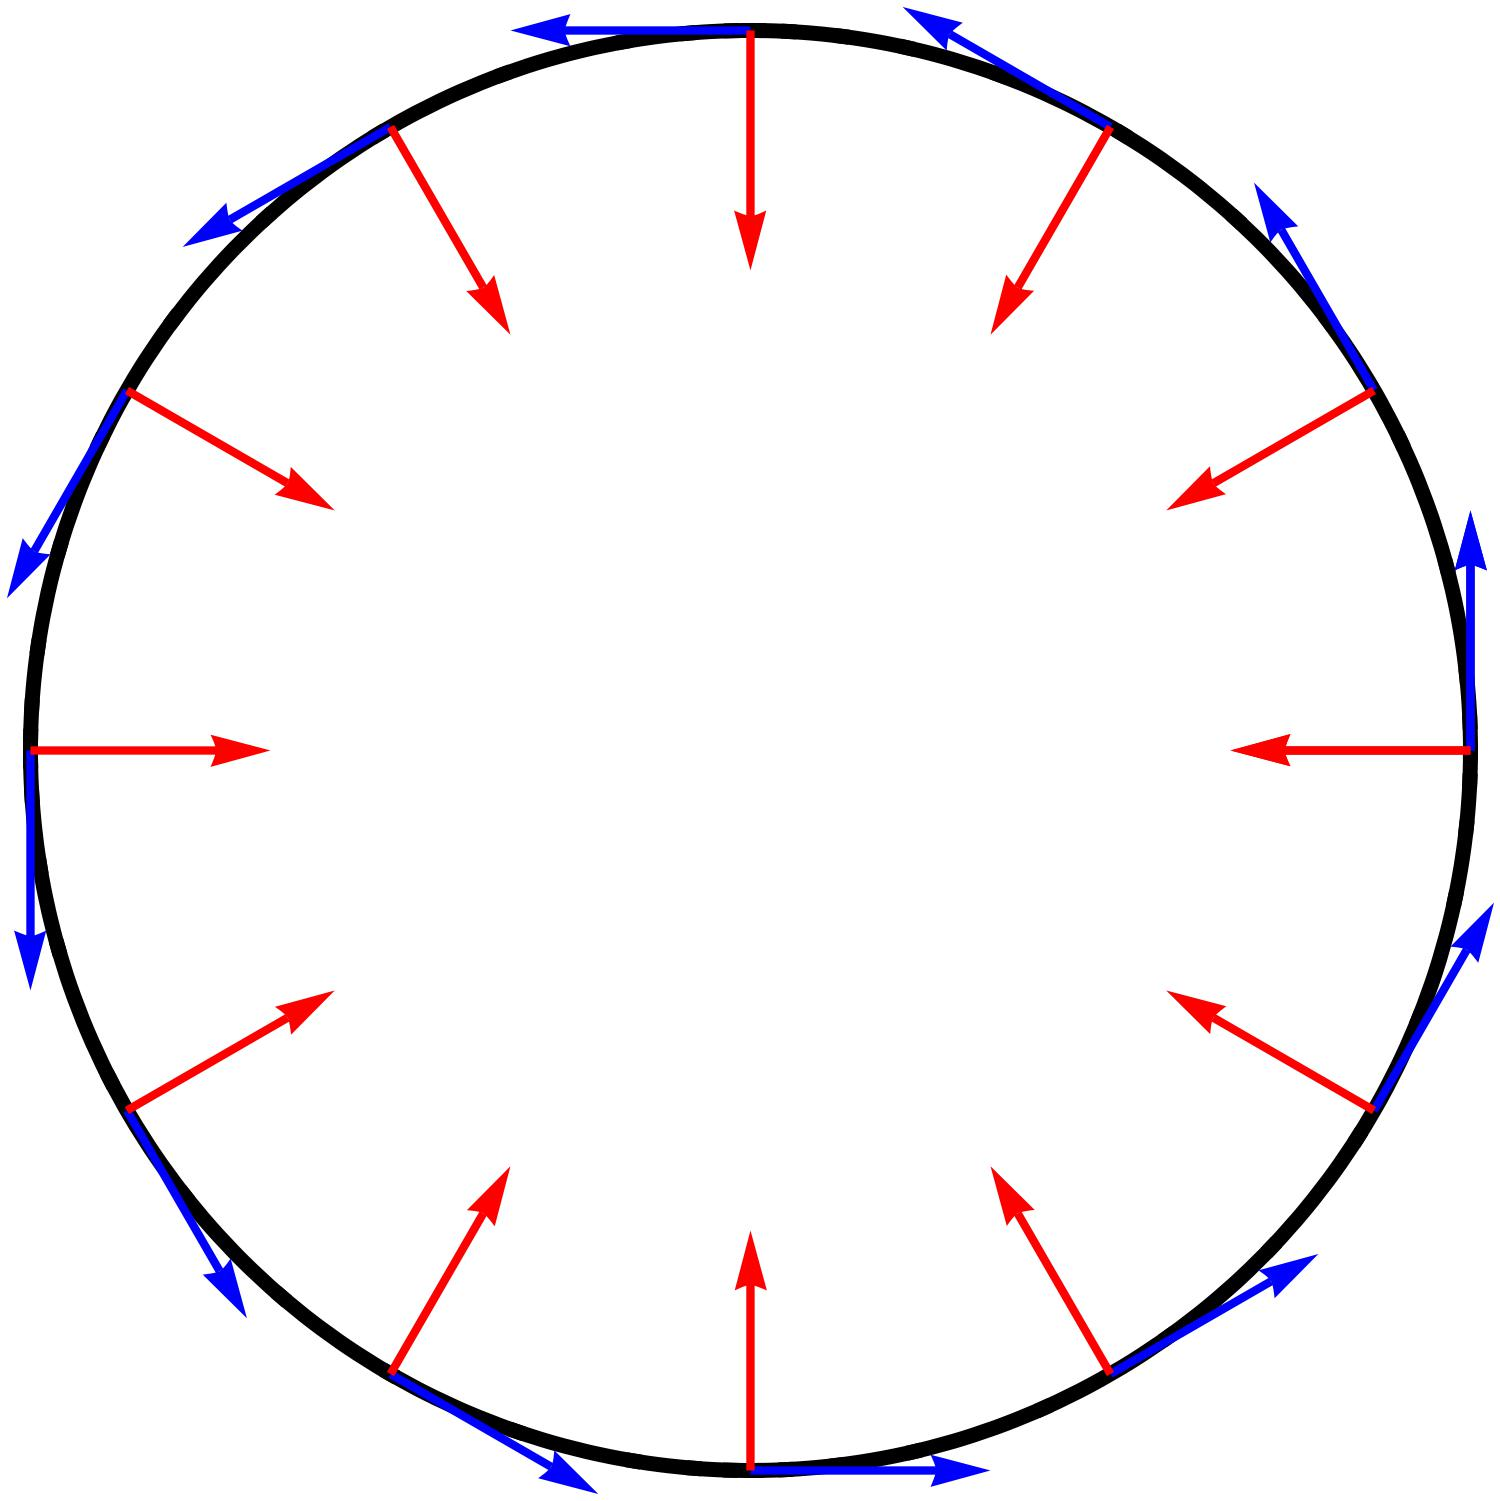
\includegraphics{circleArrows.jpg}
\end{image}
To add the sine curve, quite litterally, add it in:
\[
\vec{f}(t) = \vec{c}(t) + \unormal(t)\cdot \sin(t)
\]
\begin{onlineOnly}
We can confirm our construction with \sage: 
\begin{sageCell}
var('s t')
x(t) = 3*cos(t)
y(t) = 3*sin(t)
c(t) = (x(t),y(t))
dc=derivative(c,t)
ut= dc / dc.norm()
ddc = derivative(ut,t)
n = ddc / ddc.norm()
circle=parametric_plot(c(t),(t,0,2*pi),color="black")
curve=parametric_plot(c(t) + n*sin(5*t), (t,0,2*pi))
circle+curve
\end{sageCell}
\end{onlineOnly}
  \end{explanation}
\end{example}

\section{Thickening a curve}

Suppose you have a vector-valued function $\vec{f}:\R\to\R^2$ that
defines a curve in space, and you want to build a parameterized
surface that looks like a ``thickened'' version of the curve.  In
other words, we want to convert a curve like
\begin{image}
  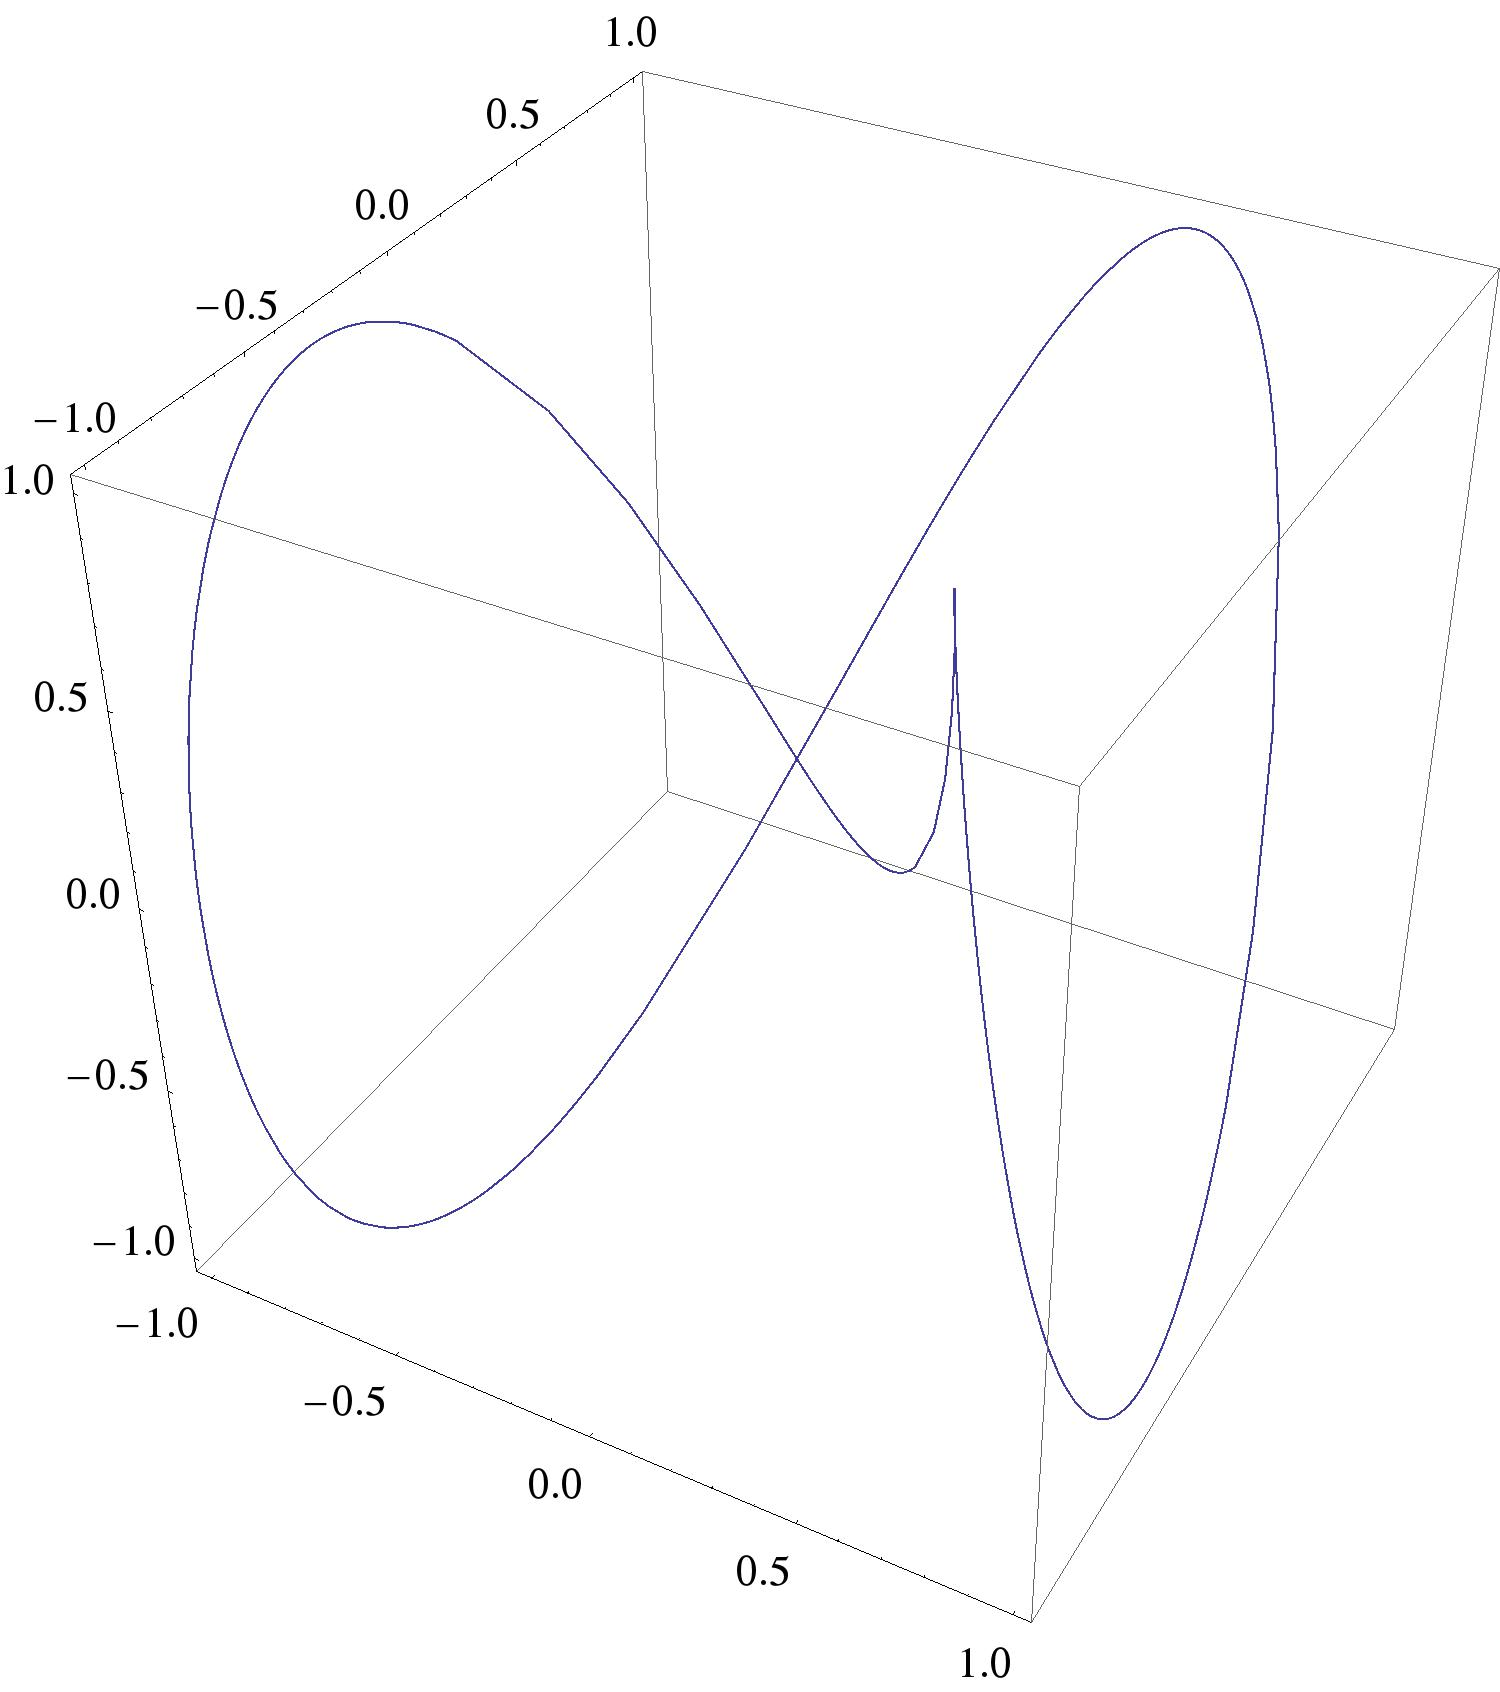
\includegraphics{curve.jpg}
\end{image}
%% \begin{sageOutput}
%% x(t) = sin(t)
%% y(t) = sin(2*t + pi/5)
%% z(t) = sin(3*t + pi/7)
%% f(t) = (x(t),y(t),z(t))
%% parametric_plot3d(f(t), (t,0,2*pi))
%%   \end{sageOutput}
into a thickened ``tube'' like
\begin{image}
  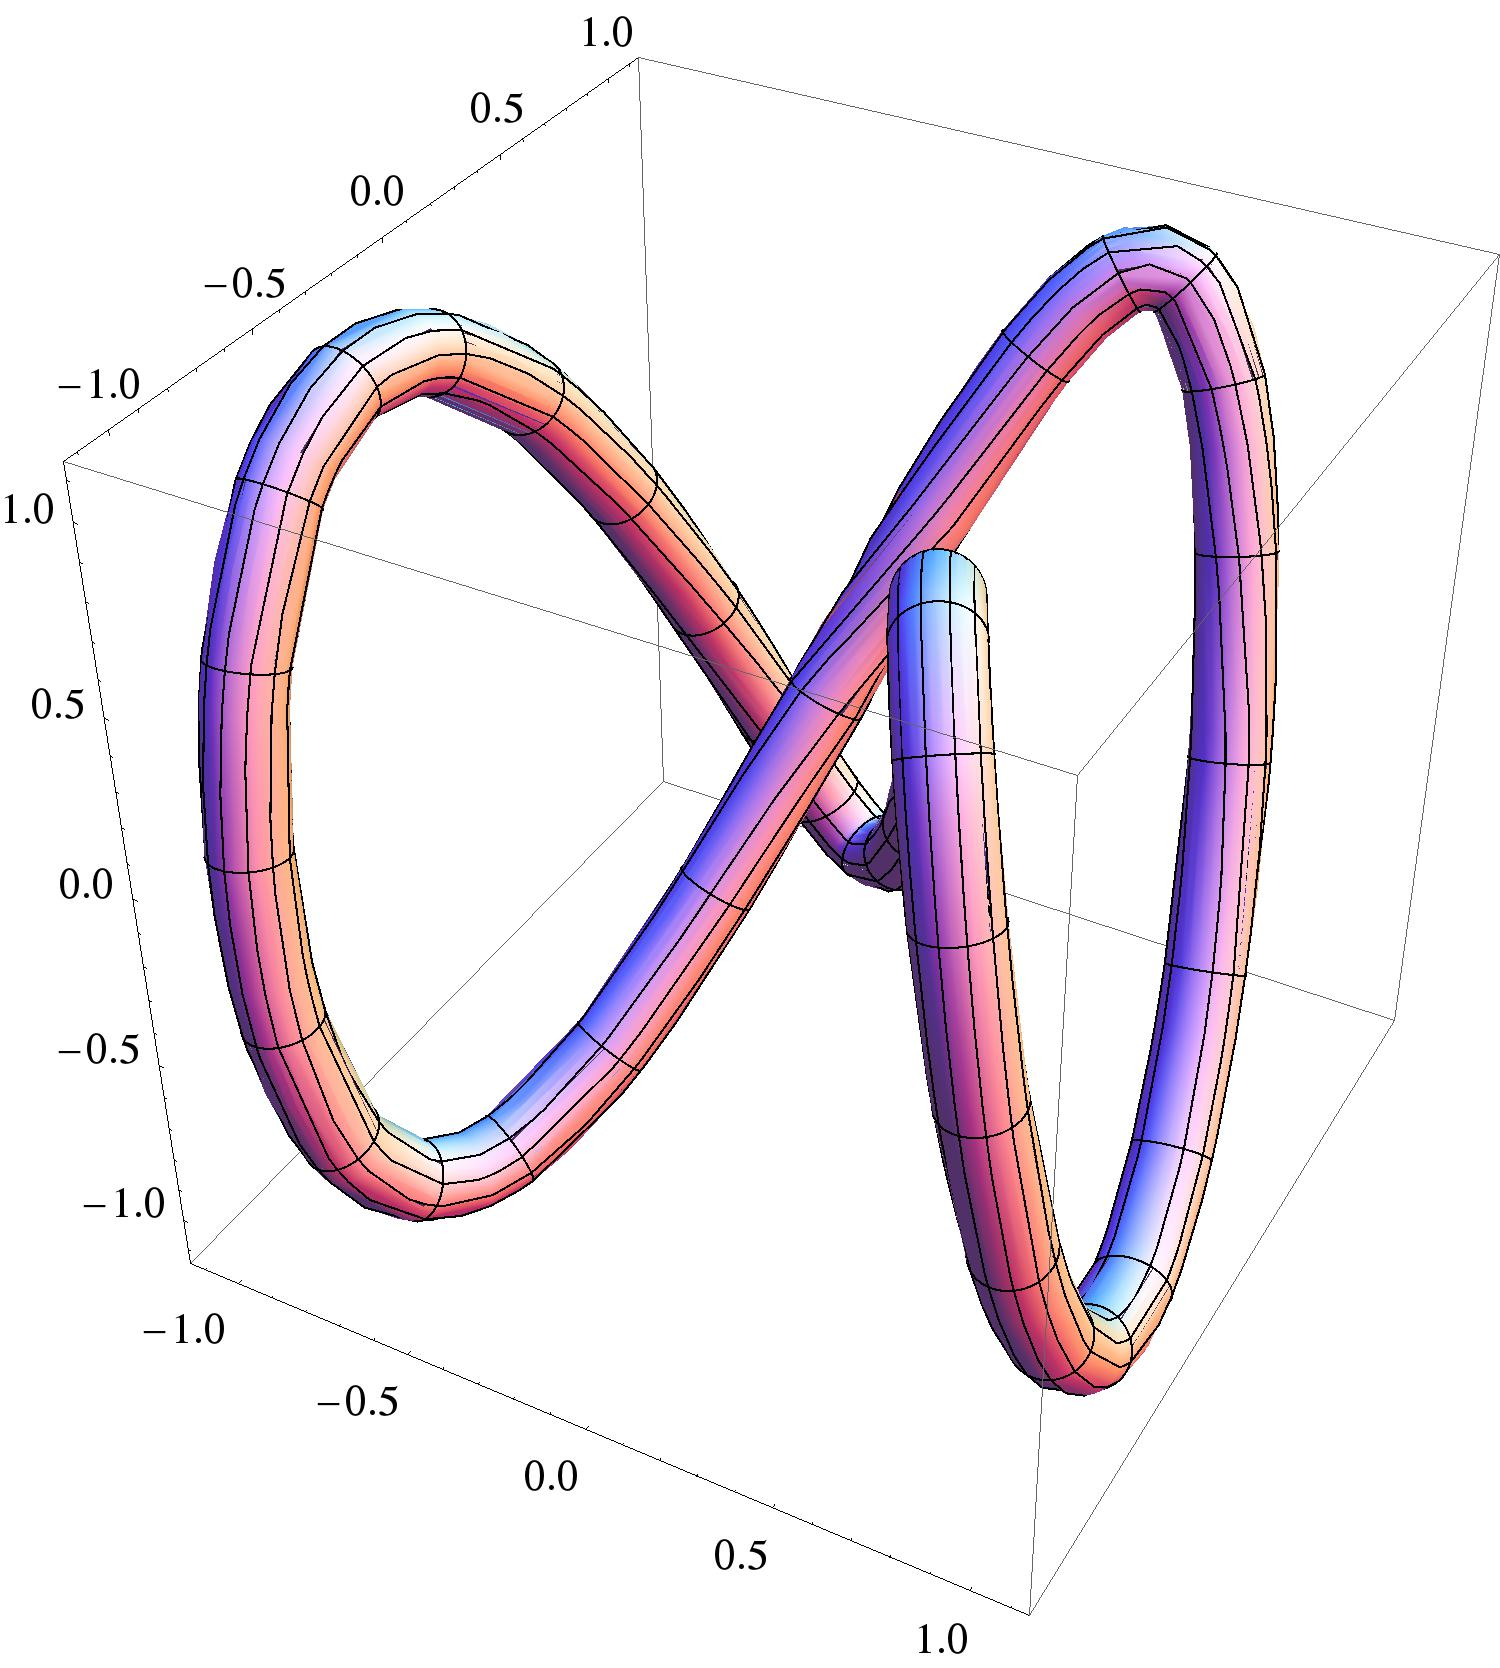
\includegraphics{tube.jpg}
\end{image}
%% \begin{sageOutput}
%% var('s')
%% x(t) = sin(t)
%% y(t) = sin(2*t + pi/5)
%% z(t) = sin(3*t + pi/7)
%% f(t) = (x(t),y(t),z(t))
%% df=derivative(f,t)
%% ut = df / df.norm()
%% ddf = derivative(ut,t)
%% n = ddf / ddf.norm()
%% bn = n.cross_product(ut)
%% thickness = 0.10
%% parametric_plot3d(f(t) + (n * cos(s) + bn * sin(s)) * thickness, (t,0,2*pi), (s,0,2*pi), plot_points=[100,100])
%%   \end{sageOutput}
%% \begin{image}
%%   \begin{tikzpicture}
%%     \begin{axis}[tick label style={font=\scriptsize},axis on top,view={-30}{30},no markers,zmax=1,axis lines=center,
%%         ymax=1.5,ymin=-1.5,clip=false,
%%         xmax=1.5,xmin=-1.5,
%%         every axis x label/.style={at={(axis cs:\pgfkeysvalueof{/pgfplots/xmax},0,0)},xshift=-3pt,yshift=-3pt},
%% 	xlabel={\scriptsize $x$},
%% 	every axis y label/.style={at={(axis cs:0,\pgfkeysvalueof{/pgfplots/ymax},0)},xshift=0pt,yshift=-5pt},
%% 	ylabel={\scriptsize $y$},
%% 	every axis z label/.style={at={(axis cs:0,0,\pgfkeysvalueof{/pgfplots/zmax})},xshift=0pt,yshift=4pt},
%% 	zlabel={\scriptsize $z$}]
%%       \addplot3+[domain=-0:360,samples=200,samples y=0,ultra thick](sin(x),{sin(2*x+36},{sin(3*x+25)});
%%     \end{axis}
%%   \end{tikzpicture}
%% \end{image}

To plot a ``tube'' around a vector-valued function $\vec{f}$, we need
three handy vectors:
\begin{itemize}
\item The \dfn{unit tangent vector}:
  \[
  \utan(t) = \frac{\vec{f}'(t)}{|\vec{f}'(t)|}
  \]
\item The \dfn{unit normal vector}:
  \[
  \unormal(t) = \frac{\vec{t}'(t)}{|\vec{t}'(t)|}
  \]
\item The \dfn{unit binormal vector}:
  \[
  \ubinormal(t) = \utan(t) \cross \unormal(t)
  \]
\end{itemize}

Let's see these vectors in action with our next example.

\begin{example}
  You have been given a curve in space, say
  \[
  \vec{f}(t) = \langle t^2-2, t^2-2, 1-t\rangle.
  \]
  We want to make a tube around it of radius $0.5$.
  \begin{explanation}
    Here is the idea, we want to take our curve and attach two
    orthogonal vectors to every point
    \begin{image}
      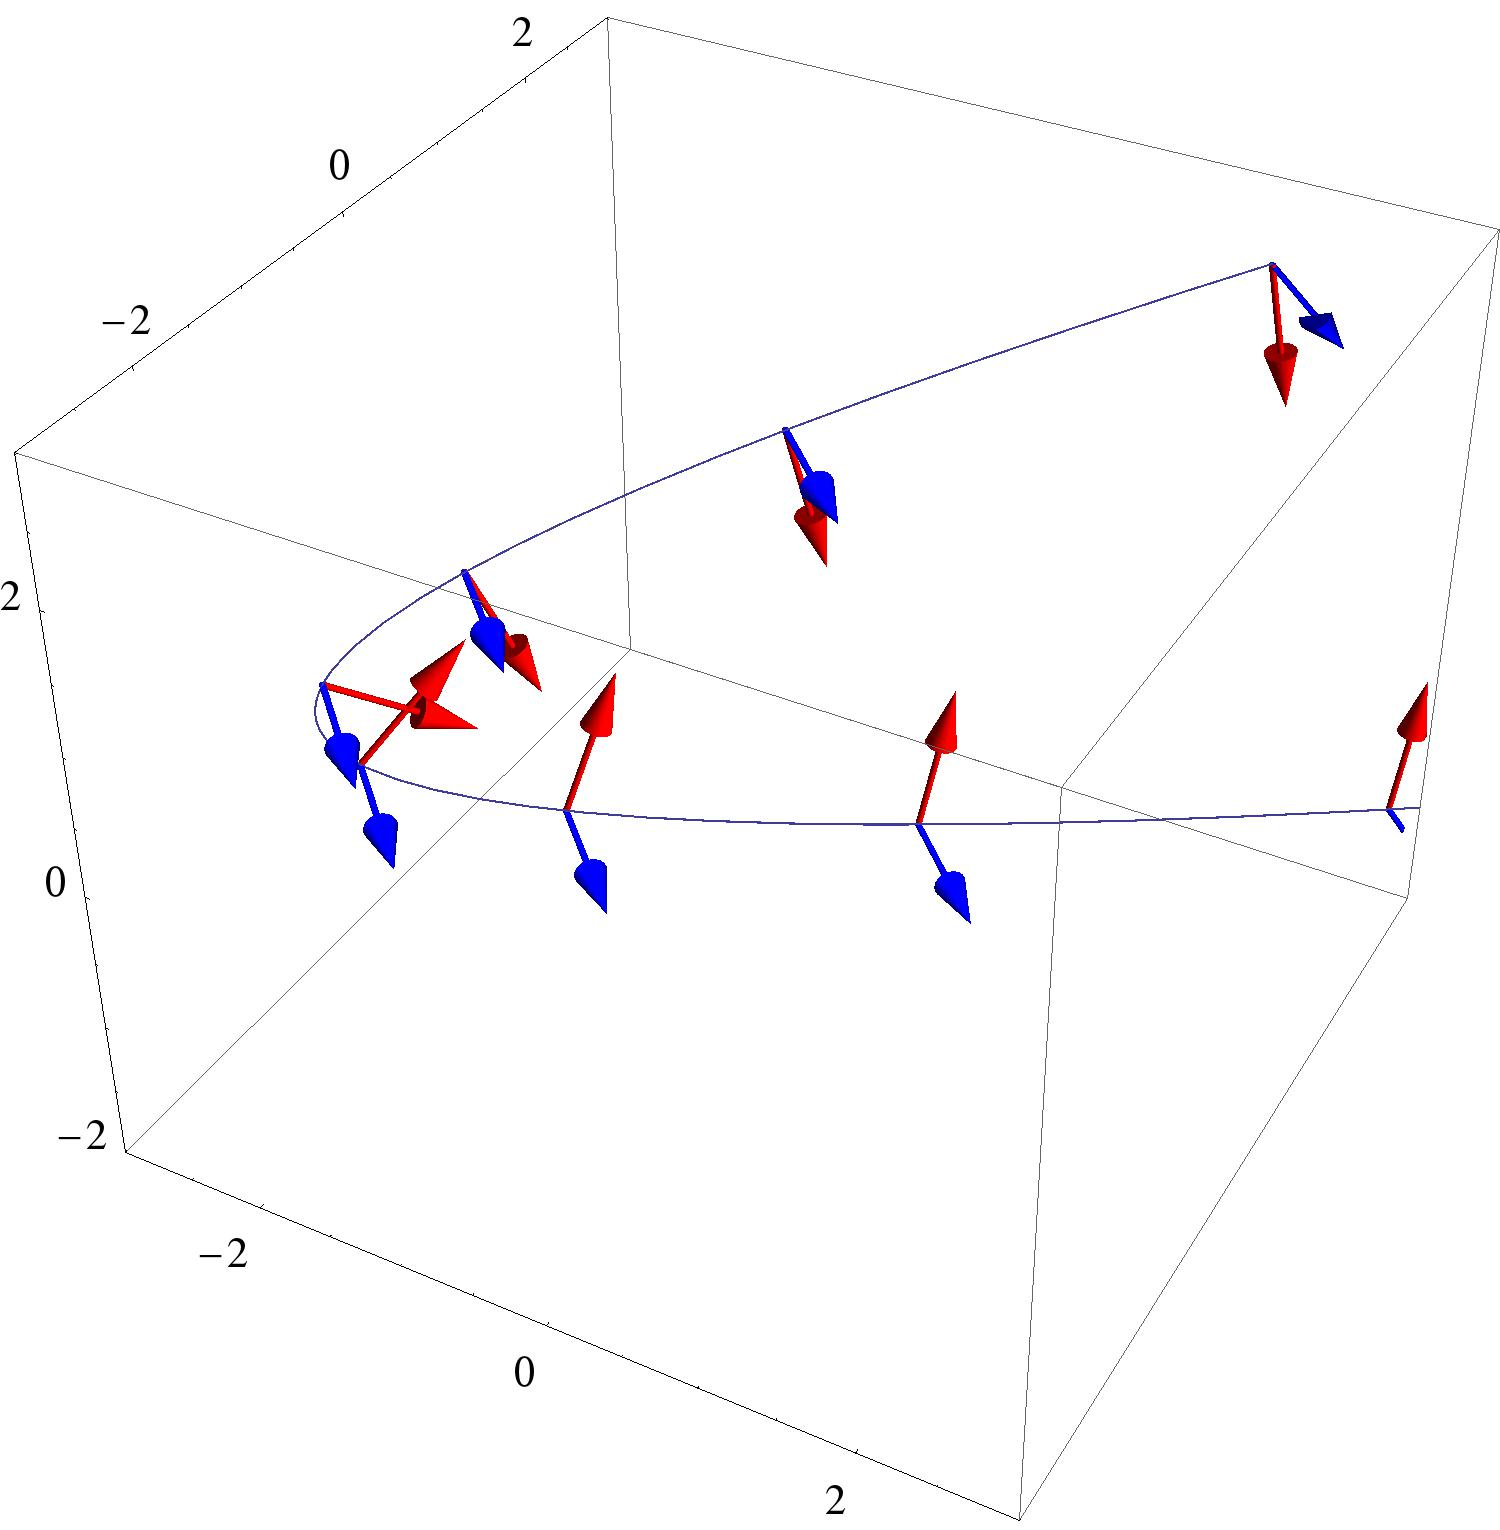
\includegraphics{paraArrows.jpg}
    \end{image}
    We'll start by computing the
    \wordChoice{\choice[correct]{unit tangent}\choice{unit normal}\choice{unit binormal}}
    vectors. Write with me
    \[
    \utan(t) = \frac{\vec{f}'(t)}{|\vec{f}'(t)|}
    \]
    From these vectors we can obtain the \wordChoice{\choice{unit
        tangent}\choice[correct]{unit normal}\choice{unit binormal}}
    vectors by differentiating:
    \[
    \unormal(t) = \frac{\utan'(t)}{|\utan'(t)|}
    \]
    Finally we can obtain the \wordChoice{\choice{unit
        tangent}\choice{unit normal}\choice[correct]{unit binormal}}
    vectors via the cross product:
    \[
    \ubinormal(t) = \utan(t) \cross \unormal(t)
    \]
    Looking again at
    \begin{image}
      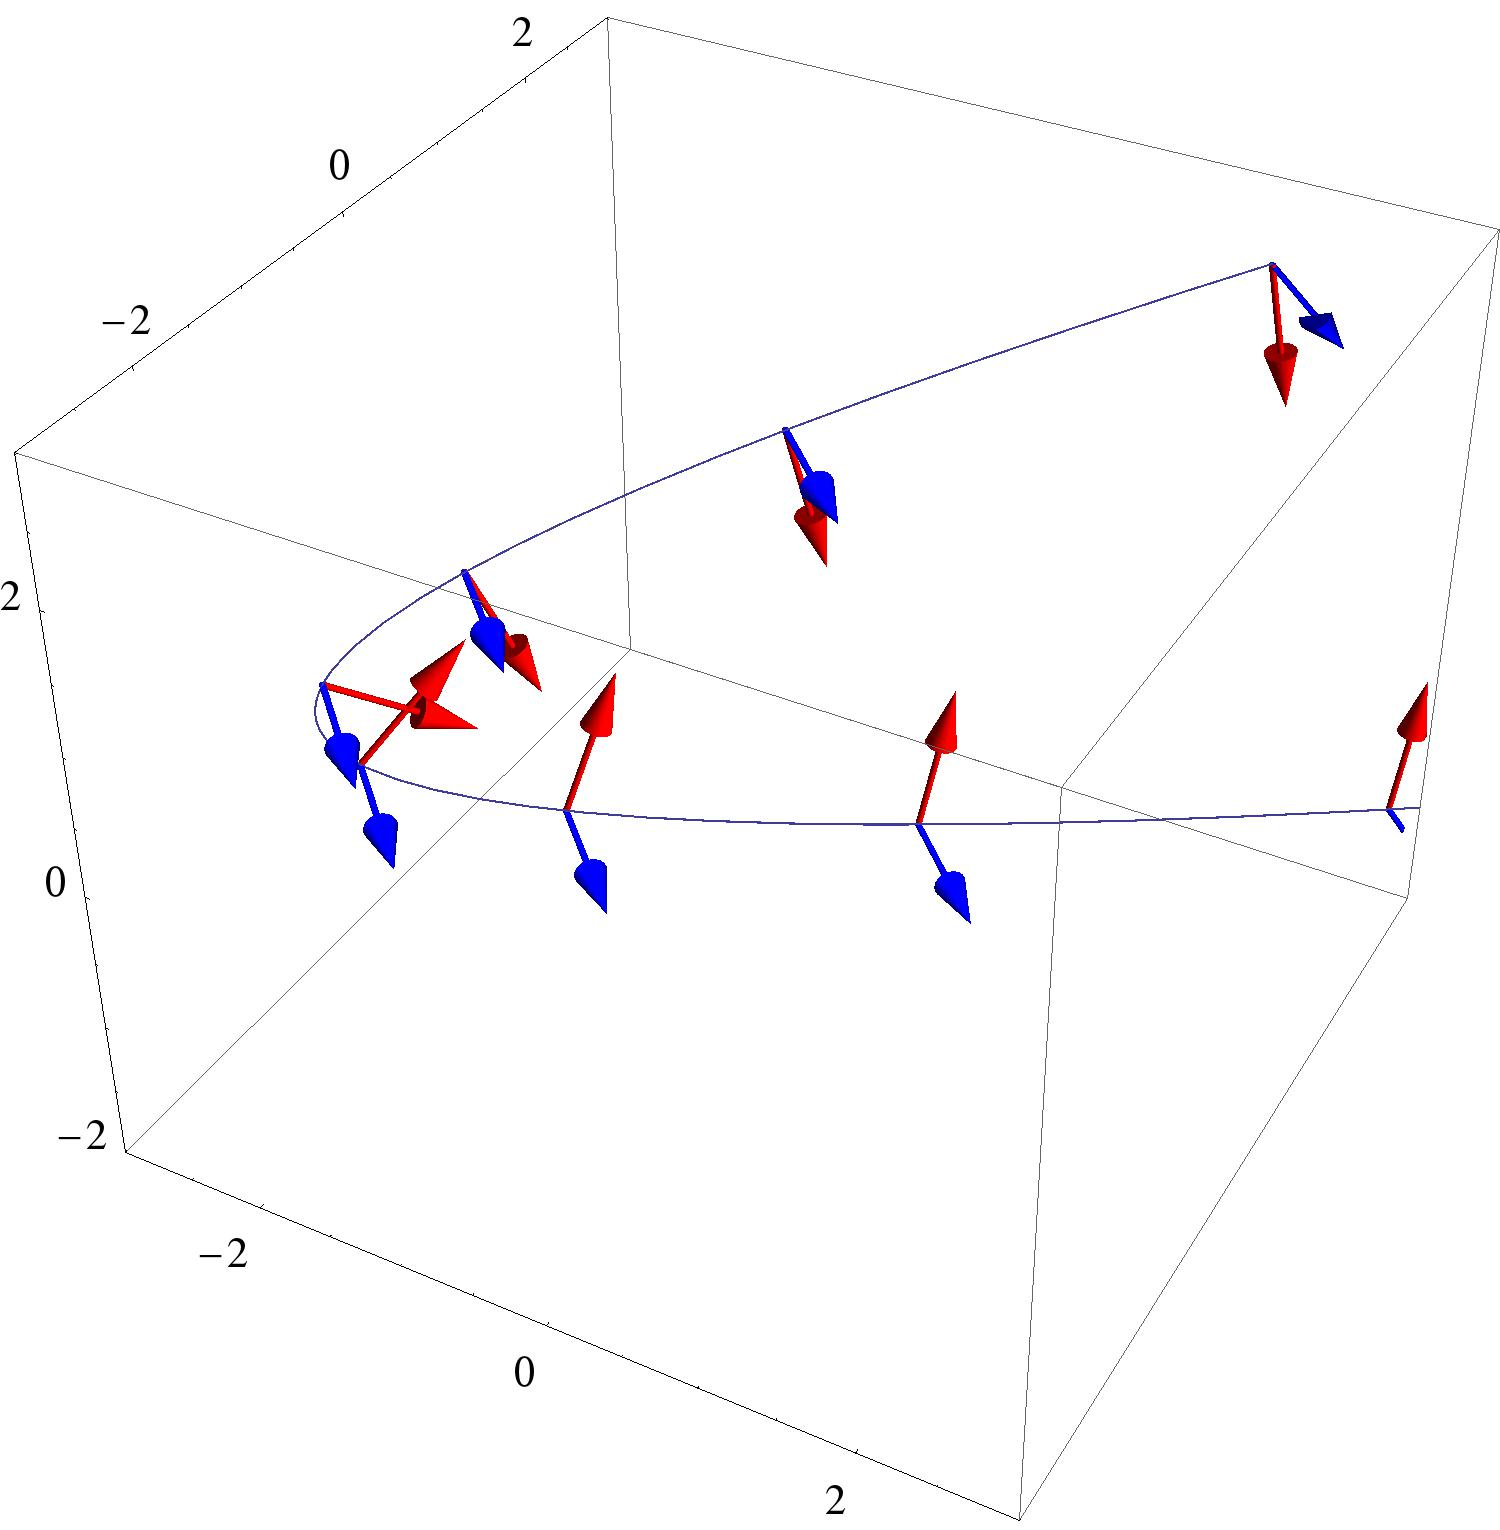
\includegraphics{paraArrows.jpg}
    \end{image}
    we see the unit normal vectors in red, and the unit binormal
    vectors in blue. So we now can plot our tube where $s$ runs from
    $0$ to $2\pi$:
    \begin{align*}
      \vec{F}(s,t) = \vec{f}(t) &+ 0.5 \unormal(\answer[given]{t})\cos(\answer[given]{s})\\
      &+ 0.5 \ubinormal(\answer[given]{t})\sin(\answer[given]{s})
    \end{align*}
    \begin{onlineOnly}
      We can check our work with \sage.
  \begin{sageCell}
var('s t')
x(t) = t^2-2
y(t) = t^2-2
z(t) = 1-t
f(t) = (x(t),y(t),z(t))
df=derivative(f,t)
ut = df / df.norm()
ddf = derivative(ut,t)
n = ddf / ddf.norm()
bn = ut.cross_product(n)
parametric_plot3d(f(t) + 0.5*n*cos(s) + 0.5*bn*sin(s), (t,-3,3), (s,0,2*pi))
  \end{sageCell}
    \end{onlineOnly}
  \end{explanation}
\end{example}


\end{document}
